\section{Double Clipping}
\label{chap2-sec:double_clip}

% However, 
% all of our three algorithms still suffer from a very large estimation error. due to a large amount of the Laplacian noise. 
In Section~\ref{chap2-sec:algorithms}, 
% \ref{chap2-sub:algorithms_theoretical_analysis}, 
we showed that the estimation error caused by empirical estimation (i.e., the first term in Theorem~\ref{chap2-thm:l2loss_algorithms}) is significantly reduced by the $4$-cycle trick. 
However, 
% all of the upper-bounds in 
the estimation error is 
% caused by the Laplacian noise (i.e., the second term)  
% Theorem~\ref{chap2-thm:l2loss_algorithms} are 
still very large in our algorithms presented in Section~\ref{chap2-sec:algorithms}, as shown in our experiments. 
% due to a large amount of the Laplacian noise (as shown in our experiments). 
% In particular, 
This is because 
the estimation error by the Laplacian noise (i.e., the second term in Theorem~\ref{chap2-thm:l2loss_algorithms}) 
% the Laplacian noise 
is very large, especially for small $\epsilon_2$ or 
% $\mu_F$ ($=\mu_O^2 = \mu_T^3$), 
$\mu$. 
% as shown in Theorem~\ref{chap2-thm:l2loss_algorithms}. 
% In Section~\ref{chap2-sec:double_clip}, we introduce a double clipping technique to significantly reduce the amount of Laplacian noise.
This error term is tight and unavoidable as long as we use $d_{max}$ as a global sensitivity, which suggests that we need a better global sensitivity analysis.
% In 
% Section~\ref{chap2-sec:double_clip}, 
% the next section, 
% we introduce \textit{double clipping} to significantly reduce the amount of Laplacian noise.
% 
% Our three algorithms in Section~\ref{chap2-sec:algorithms} suffer from a large amount of the Laplacian noise. 
% due to the large global sensitivity. 
% To address this issue, 
% Thus, we propose a double clipping technique, which significantly reduces the global sensitivity of the Laplacian noise. 
To significantly reduce the global sensitivity, we propose a novel \textit{double clipping} technique. 
% Therefore, we propose a double clipping technique, which significantly reduces the global sensitivity of the Laplacian noise. 

We describe the overview and details of our double clipping in Sections~\ref{chap2-sub:clip_overview} and \ref{chap2-sub:algorithms}, respectively. 
Then we perform theoretical analysis in Section~\ref{chap2-sub:clip_theoretical_analysis}.

\subsection{Overview}
\label{chap2-sub:clip_overview}

% \smallskip
\noindent{\textbf{Motivation.}}~~Figure~\ref{chap2-fig:reduce_noisy_triangles} shows noisy triangles involving edge $(v_i,v_j)$ counted by user $v_i$ in our three algorithms. 
Our algorithms in Section~\ref{chap2-sec:algorithms} 
% (and the two-rounds algorithm in \cite{Imola_USENIX21}) 
use the fact that the number of such noisy triangles (hence the global sensitivity) is upper-bounded by the maximum degree $d_{max}$ because 
%user $v_i$'s degree is at most $d_{max}$). 
adding one edge increases the triangle count by at most $d_{max}$. 
Unfortunately, this upper-bound is too large, as shown in our experiments. 
% Although this is correct, we 

% Our basic idea is that we can 
In this paper, we 
significantly reduce this upper-bound by using the parameter $\mu$ in the ARR and user $v_i$'s degree $d_i \in \nnints$ for users with smaller IDs. 
For example, 
% we can expect that 
the number of noisy triangles involving $(v_i,v_j)$ in \AlgOne is 
expected to be around 
$\mu d_i$ 
% ($\mu \ll 1$, $d_i < d_{max}$) 
% with high probability (larger than $0.5$) 
because one noisy edge is included in each noisy triangle (as shown in Figure~\ref{chap2-fig:reduce_noisy_triangles}) and all noisy edges are independent. 
$\mu d_i$ is very small, especially when we set $\mu \ll 1$ to reduce the communication cost.  
% Similarly, the expected number of noisy triangles involving $(v_i,v_j)$ in \AlgTwo is $\mu_O^2 d_i$ because two independent noisy edges are in each noisy triangle (as in Figure~\ref{chap2-fig:reduce_noisy_triangles}).

However, we cannot directly use $\mu d_i$ as an upper-bound of the global sensitivity in \AlgOne for two reasons. 
First, $\mu d_i$ leaks the exact value of user $v_i$'s degree $d_i$ 
and 
% , hence 
violates edge LDP. 
% friendship information of $v_i$ (e.g., as an extreme example, $d_i=0$ reveals the fact that $v_i$ has no friends). 
Second, the number of noisy triangles involving $(v_i,v_j)$ exceeds $\mu d_i$ with high probability (about $0.5$). 
Thus, the noisy triangle count cannot be upper-bounded by $\mu d_i$. 

\begin{figure}[t]
  \centering
  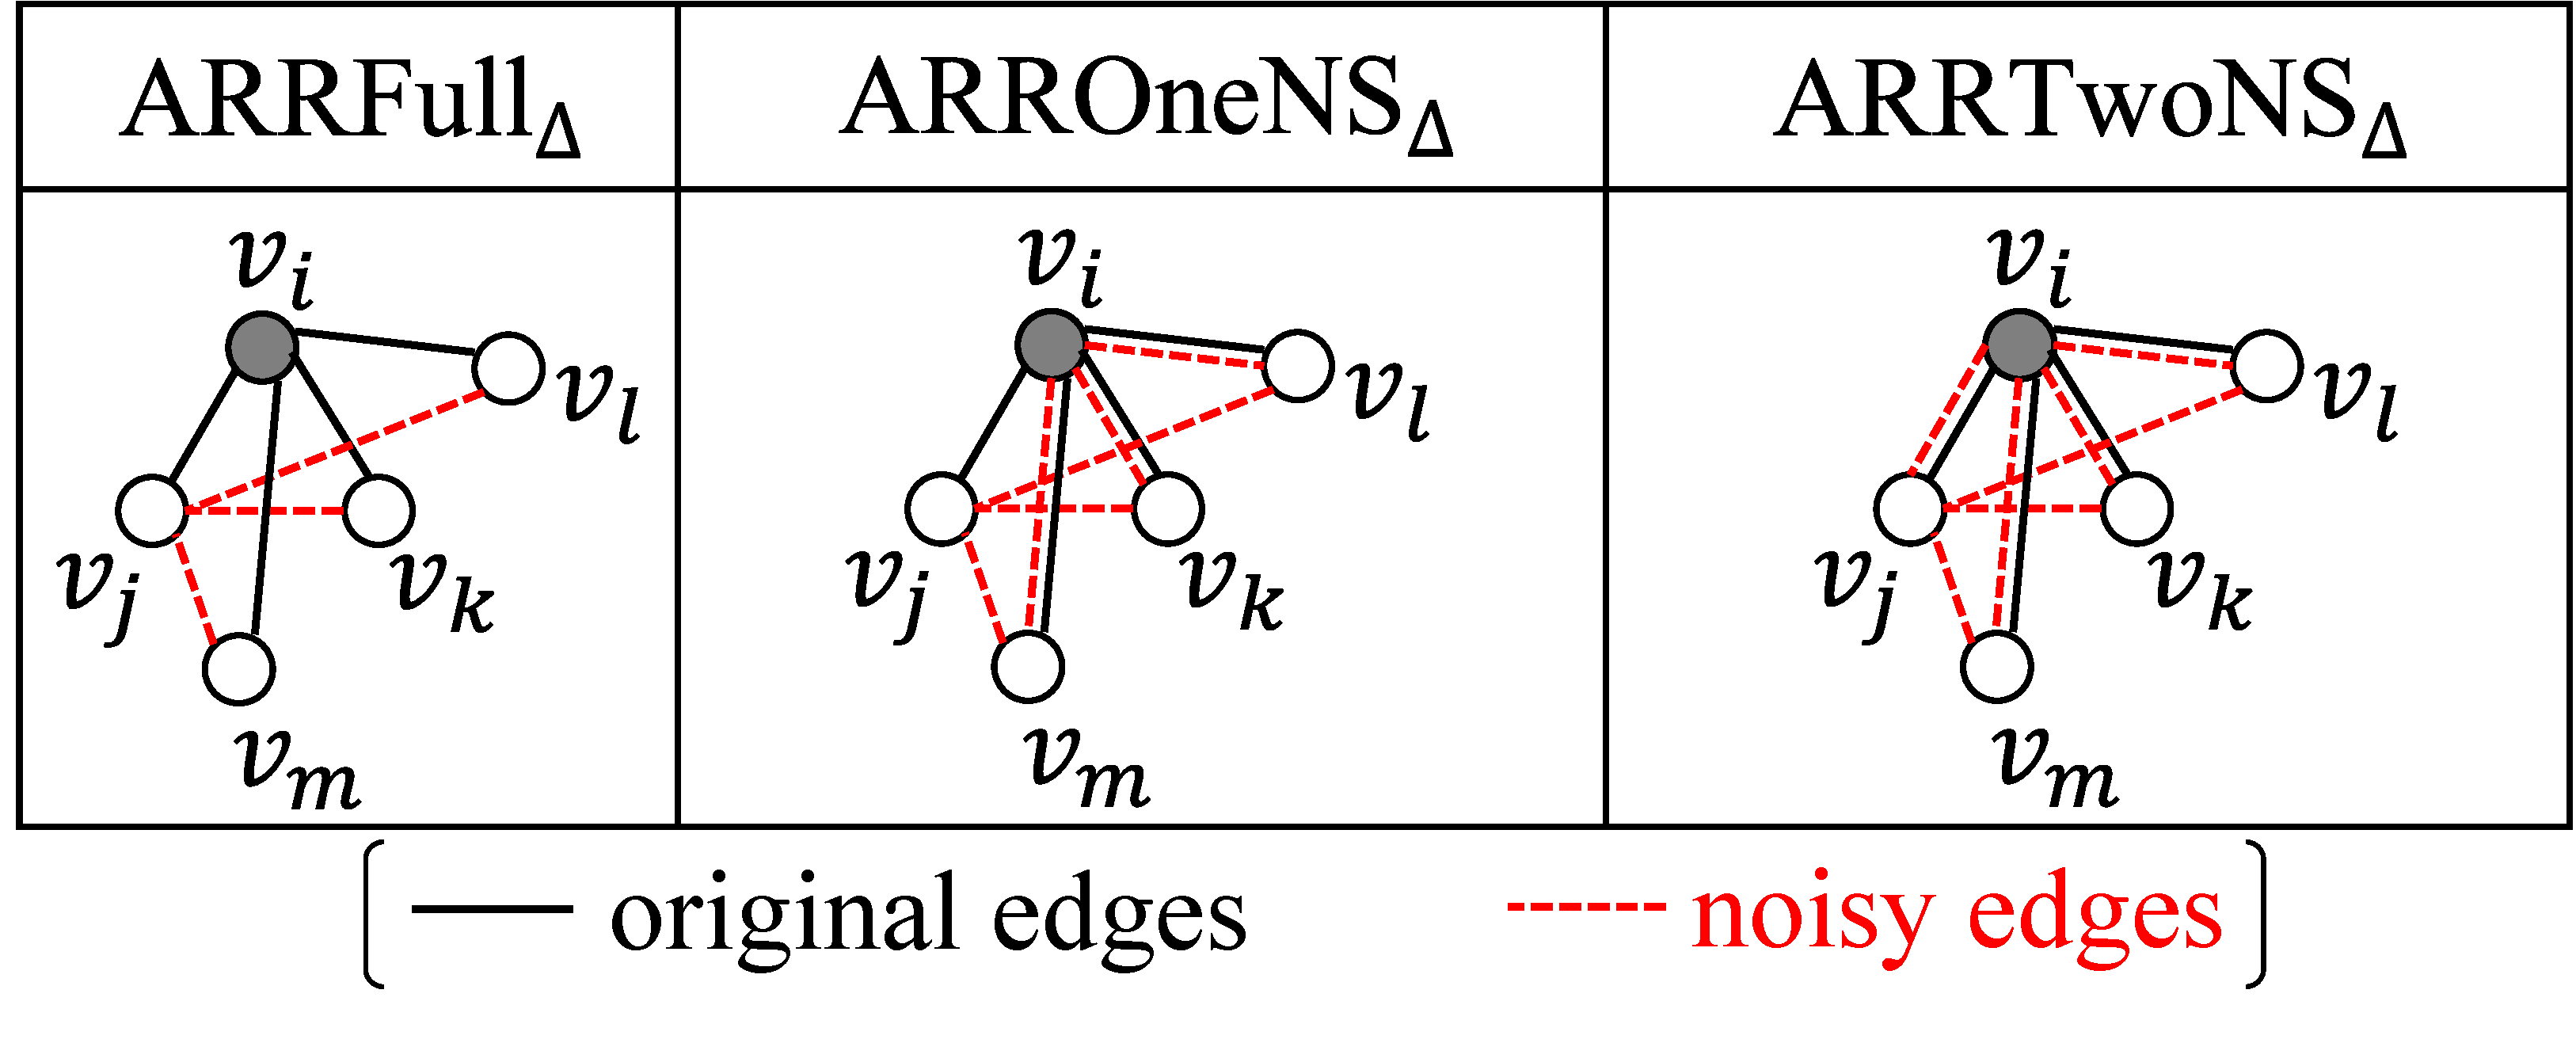
\includegraphics[width=0.78\linewidth]{fig/double_clipping.pdf}
  
  \caption[Noisy triangles involving edge $(v_i, v_j)$ counted by user $v_i$.]{Noisy triangles involving edge $(v_i,v_j)$ counted by user $v_i$ ($j<k,l,m<i$).} 
  \label{chap2-fig:reduce_noisy_triangles}
%\end{figure}
\vspace{2mm}
%\begin{figure}[t]
  \centering
  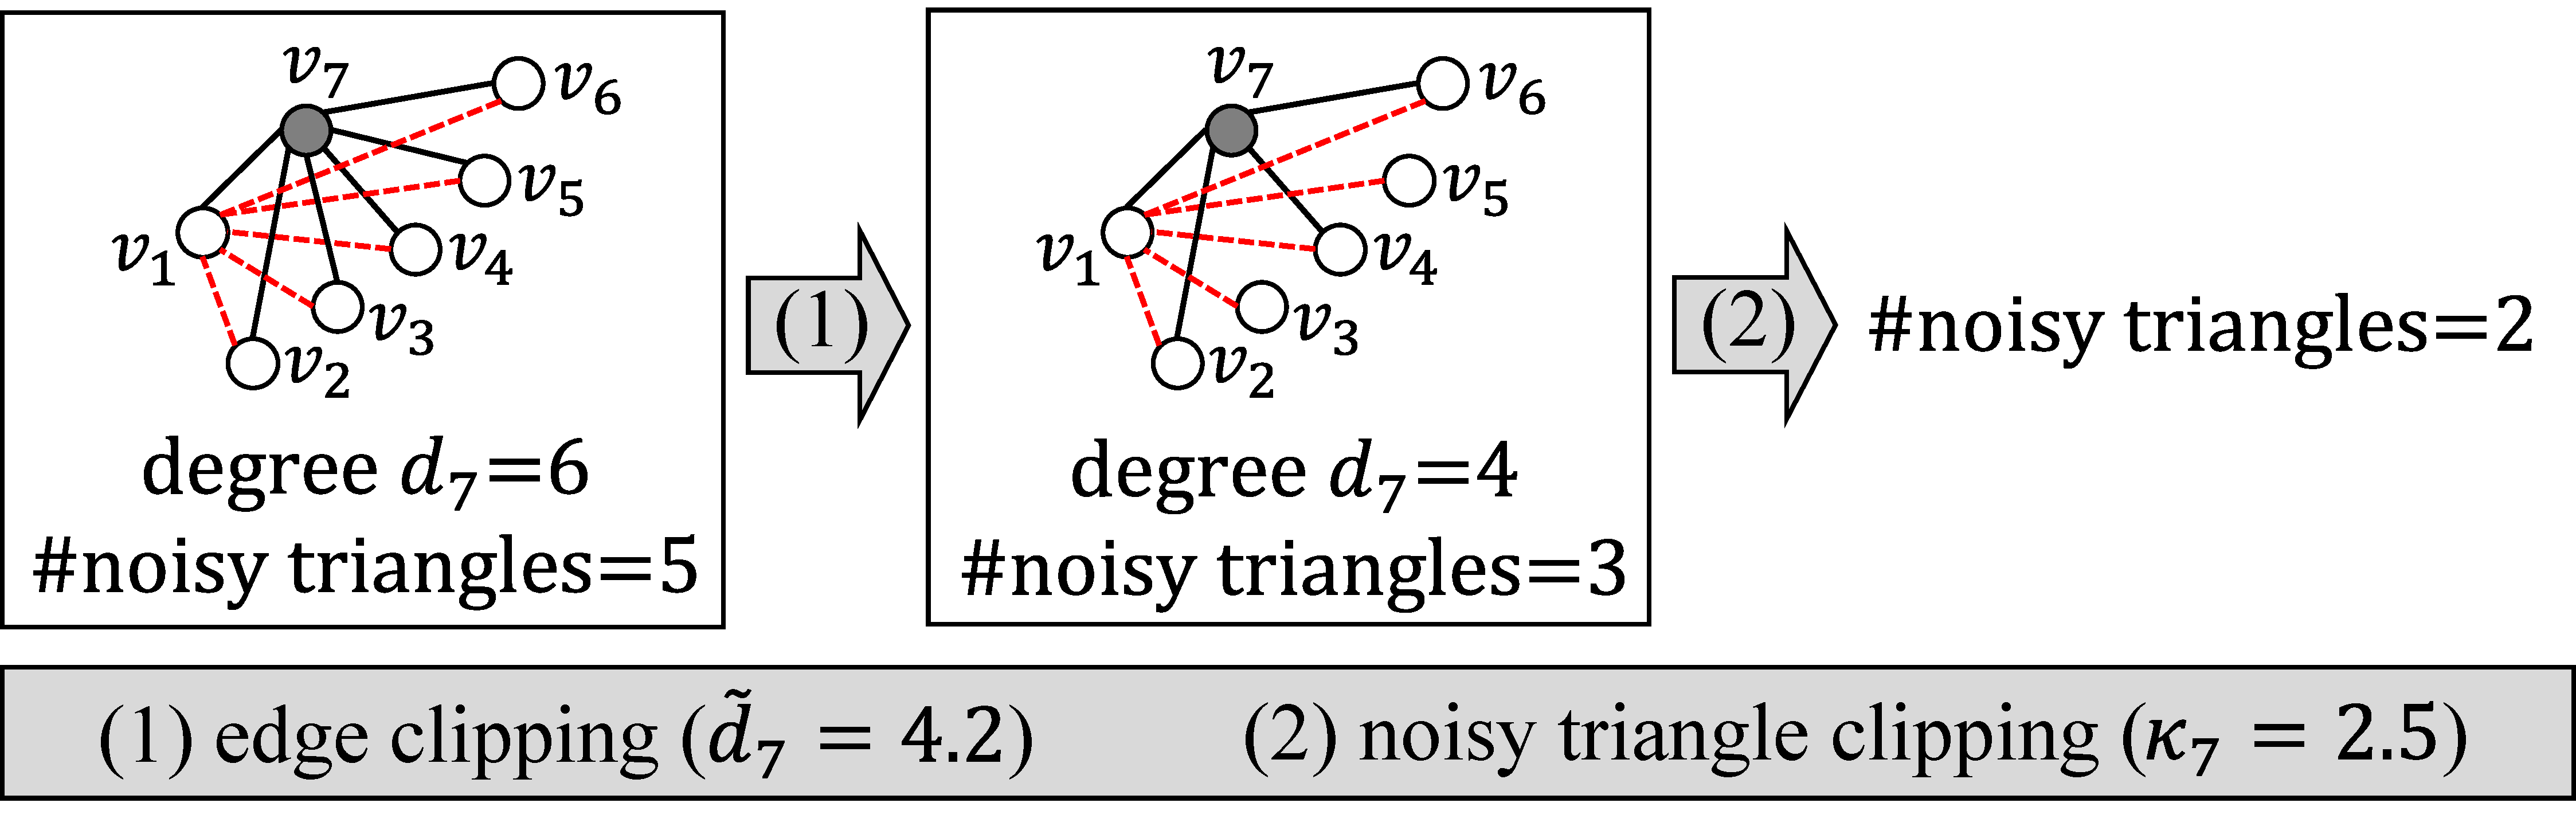
\includegraphics[width=0.99\linewidth]{fig/clip_overview.pdf}
  
  \caption[Overview od double clipping.]{Overview of double clipping applied to edge ($v_1,v_7$).} 

  \label{chap2-fig:double-clip_overview}
\end{figure}

% To address the first and second issues explained above, we introduce an edge clipping and triangle clipping, respectively. 
To address these two issues, 
%(i.e., the leakage of $d_i$ and the excess of the noisy triangle count), 
we propose a double clipping technique, which is explained below. 
% which consists of an \textit{adaptive edge clipping} and \textit{noisy triangle clipping}. 

\smallskip
\noindent{\textbf{Algorithm Overview.}}~~Figure~\ref{chap2-fig:double-clip_overview} shows 
% its overview. 
the overview of our double clipping, which consists of an 
% \textit{adaptive edge clipping} 
\textit{edge clipping} 
and \textit{noisy triangle clipping}. 
% The adaptive edge clipping 
The edge clipping 
addresses the first issue (i.e., leakage of $d_i$) 
as follows. 
% by borrowing the idea of adaptive clipping \cite{Andrew_arXiv21,Pichapati_arXiv19} 
% in DP-SGD (Differentially Private Stochastic Gradient Descent). 
% which privately estimates an appropriate clipping threshold in DP-SGD (Stochastic Gradient Descent) \cite{Abadi_CCS16} with DP. 
% Specifically, it 
It privately computes 
a noisy version of 
$d_i$ (denoted by $\td_i$) with edge LDP. 
% Let $\td_i \in \nnreals$ be the private value of $d_i$. 
% user $v_i$ 
% adds the Laplacian noise and some positive constant $\eta \in \nnreals$ to $d_i$ to provide edge LDP 
% and 
Then it 
%performs edge clipping 
%(a.k.a. graph projection \cite{Day_SIGMOD16,Ding_TKDE21,Kasiviswanathan_TCC13,Raskhodnikova_arXiv15}), which 
removes some neighbors from a neighbor list $\bma_i$ so that the degree of $v_i$ never exceeds 
% the private estimate of $d_i$. 
% the private value of $d_i$ 
% (denoted by $\td_i \in \nnreals$). 
% (denoted by $\td_i$). 
the noisy degree $\td_i$. 
This removal process is also known as graph projection \cite{Day_SIGMOD16,Ding_TKDE21,Kasiviswanathan_TCC13,Raskhodnikova_arXiv15}. 
% This kind of technique is called adaptive clipping \cite{Andrew_arXiv21,Pichapati_arXiv19} 
% in DP-SGD (Stochastic Gradient Descent) \cite{Abadi_CCS16} because it privately estimates an appropriate clipping threshold with DP. 
% Adaptive edge clipping 
Edge clipping 
is 
% also 
used in \cite{Imola_USENIX21} to obtain a 
% private value of 
noisy version of 
% the maximum degree 
$d_{max}$. 
%(though ours is to obtain a noisy version of $d_i$). 

% The triangle clipping addresses the second issue (i.e., excess of the noisy triangle count) by reducing the noisy triangle count so that it never exceeds a 
% user-dependent threshold $\kappa_i \in \nnints$. 
The main novelty in our double clipping lies at the \textit{noisy triangle clipping} to address the second issue (i.e., excess of the noisy triangle count). 
% Note that 
This issue appears 
% only 
when 
% each edge is sampled and 
we attempt to reduce the global sensitivity by using 
a very small sampling probability for each edge. 
% value of $\mu$ in the ARR.  
% using a stochastic algorithm such as the ARR. 
Therefore, the noisy triangle clipping has not been studied in the existing works on private triangle counting 
% \cite{Ding_TKDE21,Imola_USENIX21,Karwa_PVLDB11,Kasiviswanathan_TCC13,Song_arXiv18,Sun_CCS19,Ye_ICDE20,Ye_TKDE21,Zhang_SIGMOD15}, 
\cite{Ding_TKDE21,Imola_USENIX21,Karwa_PVLDB11,Kasiviswanathan_TCC13,Sun_CCS19,Ye_ICDE20,Ye_TKDE21,Zhang_SIGMOD15}, 
because they do not apply a sampling technique. 

Our noisy triangle clipping reduces the noisy triangle count so that it never exceeds a 
user-dependent clipping threshold 
$\kappa_i \in \nnreals$. 
% $\kappa_i = \lambda_i \mu^* \td_i$, where $\lambda_i \in \nats$. 
% We call $\kappa_i$ and $\lambda_i$ the \textit{clipping threshold} and \textit{clipping coefficient}, respectively. 
Then a crucial issue is how to set 
an appropriate 
% clipping 
threshold 
$\kappa_i$. 
We theoretically analyze the probability that the noisy triangle count exceeds $\kappa_i$ 
(referred to as the \textit{triangle excess probability}) 
as a function of 
the ARR parameter $\mu$ and the 
% private value $\td_i$ of $d_i$. 
noisy degree $\td_i$. 
% of user $v_i$. 
Then we set $\kappa_i$ so that 
the triangle excess probability 
% the probability 
is very small ($=10^{-6}$ in our experiments). 

We use the clipping threshold $\kappa_i$ as a global sensitivity. 
% of the Laplacian noise. 
Note that $\kappa_i$ provides edge LDP because $\td_i$ provides edge LDP, 
% and $\kappa_i$ depends on only $\mu$ and $\td_i$ 
i.e., immunity to post-processing \cite{DP}. 
$\kappa_i$ is also very small when $\mu \ll 1$, as it is determined based on $\mu$. 

% We also emphasize that our double clipping does \textit{not} assume that $d_{max}$ is public, because it privately computes $\td_i$. 
% by adaptive edge clipping.

\subsection{Algorithms}
\label{chap2-sub:algorithms}
Algorithm~\ref{chap2-alg:clip} shows our double clipping algorithm. 
All the processes are run by user $v_i$ at the second round. 
Thus, there is no interaction with the server in Algorithm~\ref{chap2-alg:clip}.

\setlength{\algomargin}{5mm}
\begin{algorithm}[t]
  \SetAlgoLined
  \KwData{Neighbor list $\bma_i \in \{0,1\}^n$, privacy budget
  $\epsilon_0 \in \nnreals$ 
  $\mu \in [0,\frac{e^{\epsilon_1}}{e^{\epsilon_1} + 1}]$, 
  %$\eta \in \nnreals$.
  $\alpha \in \nnreals$, 
  $\beta \in \nnreals$.
  }
  \KwResult{$\hw_i$.}
  $\mu^* \leftarrow \mu$, $\mu^2$, and $\mu^3$ in F, O, and T, respectively\;
  \tcc{Edge clipping.}
  %$\td_i = \max\{d_i + \Lap(\frac{1}{\epsilon_0}) + \eta$, 0\}\;
  $\td_i = \max\{d_i + \Lap(\frac{1}{\epsilon_0}) + \alpha$, 0\}\;
  \tcc{Remove $d_i - \lfloor \td_i \rfloor$ neighbors if $d_i > \td_i$.}
  $\bma_i \leftarrow \texttt{GraphProjection}(\bma_i, \td_i)$\;
  \tcc{Noisy triangle clipping.}
  \For{$j$ \rm{such that} $a_{i,j} = 1$ \rm{and} $j<i$}{
    $t_{i,j} \leftarrow |\{(v_i,v_j,v_k) : a_{i,k} = 1, (v_j,v_k) \in M_i, j<k<i \}|$\;
  }
%  \tcc{Calculate $\kappa_i$ such that $\kappa_i \in [\mu^* \td_i, \td_i]$.}
   \tcc{Calculate $\kappa_i \in [\mu^* \td_i, \td_i]$ s.t. the triangle excess probability is $\beta$ or less.}
%  \tcc{Calculate $\lambda_i \in \nats$ such that the triangle excess probability is $\beta$ or less.}
  $\kappa_i \leftarrow \texttt{ClippingThreshold}(\mu, \td_i, \beta)$\;
%  $\lambda_i \leftarrow \texttt{ClippingThreshold}(\mu, \td_i, \beta)$\;
%   $\kappa_i \leftarrow \lambda_i \mu^* \td_i$\;
  $t_i \leftarrow \sum_{a_{i,j} = 1, j<i} \min \{t_{i,j}, \kappa_i\}$\;
  $s_i \leftarrow |\{(v_i,v_j,v_k) : a_{i,j} = a_{i,k} = 1, j<k<i\}|$\;
  $w_i \leftarrow t_i - \mu^* \rho s_i$\;
  $\hw_i \leftarrow w_i + \Lap(\frac{\kappa_i}{\epsilon_2})$\;
  \KwRet{$\hw_i$}
  \caption[Our double clipping algorithm.]{Our double clipping algorithm. 
  ``F'', ``O'', ``T'' are shorthands for 
  \AlgOne{}, \AlgTwo{}, and \AlgThree{}, respectively.
  All the processes are run by user $v_i$.
  }\label{chap2-alg:clip}
\end{algorithm}

\smallskip
\noindent{\textbf{Edge Clipping.}}~~The edge clipping appears in lines 2-3 of Algorithm~\ref{chap2-alg:clip}. 
It uses a privacy budget $\epsilon_0 \in \nnreals$. 
% for privately computing $d_i$. 

In line 2, user $v_i$ adds the Laplacian noise $\Lap(\frac{1}{\epsilon_0})$ to her degree $d_i$. 
Since adding/removing one edge changes $d_i$ by at most $1$, this process provides $\epsilon_0$-edge LDP. 
$v_i$ also adds some non-negative constant 
% $\eta \in \nnreals$ 
$\alpha \in \nnreals$ 
to $d_i$. 
We add this value so that edge removal (in line 3) occurs with a very small probability; 
e.g., in our experiments, we set $\alpha = 150$, where 
% when $\epsilon_0 = 0.1$ and $\alpha = 150$, 
edge removal occurs with probability $1.5 \times 10^{-7}$ when $\epsilon_0 = 0.1$. 
A similar technique is introduced in \cite{Sun_CCS19} to provide ($\epsilon, \delta)$-DP \cite{DP} with small $\delta$. 
The difference between ours and \cite{Sun_CCS19} is that we perform edge clipping 
% (graph projection) 
to always provide $\epsilon$-DP; i.e., $\delta = 0$.
Let $\td_i \in \nnreals$ be the noisy degree of $v_i$.

In line 3, user $v_i$ calls the function \texttt{GraphProjection}, which performs graph projection as follows; 
if $d_i > \td_i$, randomly remove $d_i - \lfloor \td_i \rfloor$ neighbors from $\bma_i$; otherwise, do nothing. 
Consequently, the degree 
% $d_i$ 
of $v_i$ never exceeds $\td_i$. 

\begin{table*}[t]
  \centering
	\rotatebox{270}{
  \begin{tabular}{|l|c|c|c|}
    \hline
    & \AlgOne & \AlgTwo & \AlgThree \\ \hline
    Privacy 
    & \multicolumn{3}{|c|}{$(\epsilon_0 + \epsilon_1 + \epsilon_2)$-edge LDP and $(\epsilon_0 + \epsilon_1 + \epsilon_2)$-relationship DP} \\ \hline
    %& $\epsilon_0 + \epsilon_1 + \epsilon_2$ & $\epsilon_0 + \epsilon_1 + \epsilon_2$ &
    %$\epsilon_0 + \epsilon_1 + \epsilon_2$ \\ \hline
    Expected $l_2$ loss 
    % & $\frac{2 C_4(G) + S_2(G)}{\mu(1-e^{-\epsilon_1})^2}$ + $\frac{2 \sum_{i=1}^n \kappa_{i}^2}{\mu^2 (1-e^{-\epsilon_1})^2 \epsilon_2^2}$
    % & $O\left(\frac{n d_{max}^3}{\mu(1-e^{-\epsilon_1})^2} + \frac{2 \sum_{i=1}^n \lambda_{i}^2 \td_i^2}{(1-e^{-\epsilon_1})^2 \epsilon_2^2}\right)$
    & $O\left(\frac{n d_{max}^3}{\mu(1-e^{-\epsilon_1})^2} + \frac{2 \sum_{i=1}^n \kappa_{i}^2}{\mu^2(1-e^{-\epsilon_1})^2 \epsilon_2^2}\right)$
    % & $\frac{\mu(12 S_3(G) + 6 P_3(G)) + 6 S_2(G)}{\mu^2(1-e^{-\epsilon_1})^2}$ + $\frac{2 \sum_{i=1}^n \kappa_{i}^2}{\mu^4 (1-e^{-\epsilon_1})^2 \epsilon_2^2}$
    % & $O\left(\frac{n d_{max}^2}{\mu^2(1-e^{-\epsilon_1})^2} + \frac{2 \sum_{i=1}^n \lambda_{i}^2 \td_i^2}{(1-e^{-\epsilon_1})^2 \epsilon_2^2} \right)$
    & $O\left(\frac{n d_{max}^2}{\mu^2(1-e^{-\epsilon_1})^2} + \frac{2 \sum_{i=1}^n \kappa_{i}^2}{\mu^4 (1-e^{-\epsilon_1})^2 \epsilon_2^2} \right)$
    % & $\frac{\mu^2 (12 S_3(G) + 6 P_3(G)) + 6 S_2(G)}{\mu^3(1-e^{-\epsilon_1})^2}$ + $\frac{2 \sum_{i=1}^n \kappa_{i}^2}{\mu^6 (1-e^{-\epsilon_1})^2 \epsilon_2^2}$ \\ \hline
    % & $O\left(\frac{n d_{max}^2}{\mu^3(1-e^{-\epsilon_1})^2} + \frac{2 \sum_{i=1}^n \lambda_{i}^2 \td_i^2}{(1-e^{-\epsilon_1})^2 \epsilon_2^2} \right)$ \\ \hline
    & $O\left(\frac{n d_{max}^2}{\mu^3(1-e^{-\epsilon_1})^2} + \frac{2 \sum_{i=1}^n \kappa_{i}^2}{\mu^6 (1-e^{-\epsilon_1})^2 \epsilon_2^2} \right)$ \\ \hline
    % $l_2$ loss of emp 
    % & $\frac{2 C_4(G) + S_2(G)}{\mu_F(1-e^{-\epsilon_1})^2}$
    % & $\frac{\mu_O(12 S_3(G) + 6 P_3(G)) + 6 S_2}{\mu_O^2(1-e^{-\epsilon_1})^2}$
    % & $\frac{\mu_T^2 (12 S_3(G) + 6 P_3(G)) + 6 S_2}{\mu_T^3(1-e^{-\epsilon_1})^2}$ \\ \hline
    % $l_2$ loss of \Lap{} 
    % & $\frac{2 \sum_{i=1}^n \kappa_{i,F}^2}{\mu_F^2 (1-e^{-\epsilon_1})^2 \epsilon_2^2}$
    % & $\frac{2 \sum_{i=1}^n \kappa_{i,O}^2}{\mu_F^2 (1-e^{-\epsilon_1})^2 \epsilon_2^2}$
    % & $\frac{2 \sum_{i=1}^n \kappa_{i,T}^2}{\mu_F^2 (1-e^{-\epsilon_1})^2 \epsilon_2^2}$ \\ \hline
    $\text{Cost}_{DL}$ & 
    $\mu n^2 \log n$ 
    % $\mu e^{-\epsilon_1} n^2 \log n$ 
    % $\mu_F e^{-\epsilon_1} n(n-1) \log n$ 
    % $(n(n-1) \mu_F \rho + |E| \mu_F (1 - \rho)) \log n$ 
    & 
    $\mu^2 n^2 \log n$ 
    % $\mu^2 e^{-\epsilon_1} n^2 \log n$ 
    % $\mu_O^2 e^{-\epsilon_1} n(n-1) \log n$ 
    & 
    $\mu^3 n^2 \log n$ 
    % $\mu^3 e^{-\epsilon_1} n^2 \log n$ 
    % $\mu_T^3 e^{-\epsilon_1} n(n-1) \log n$ 
    \\ \hline
    $\text{Cost}_{UL}$ & 
    $\mu n \log n$ & $\mu n \log n$ & $\mu n \log n$ 
    % $\mu e^{-\epsilon_1} n \log n$ & $\mu e^{-\epsilon_1} n \log n$ & $\mu e^{-\epsilon_1} n \log n$ 
    \\ \hline
  \end{tabular}
	}	
  \caption[Performance gurantees of our three algorithms with double clipping when edge and triange removal do not occur.]
	{Performance guarantees 
  %Privacy, expected $l_2$ loss, and download/upload cost 
  of our three algorithms with double clipping when the edge removal and triangle removal do not occur. 
  %($C_4$: \#$4$-cycles, $P_3$: \#$3$-paths, $S_k$: \#$k$-stars). 
  %($\lambda_i$: clipping coefficient, $\td_i$: noisy degree).
  The expected $l_2$ loss assumes that $\mu$ is small. 
  The download (resp.~upload) cost is an upper-bound in (\ref{chap2-eq:CostDL_F}) 
  %, (\ref{chap2-eq:CostDL_O}), (\ref{chap2-eq:CostDL_T}), 
  (resp.~(\ref{chap2-eq:CostUL_proposal})).
  %approximation when $d_{max} \ll n$. 
  %the graph $G$ is sparse.
  }
  \label{chap2-tab:privacy_utility_cost}
\end{table*}

\smallskip
\noindent{\textbf{Noisy Triangle Clipping.}}~~The noisy triangle clipping appears in lines 4-11 of Algorithm~\ref{chap2-alg:clip}. 

% First, 
In lines 4-6, 
user $v_i$ calculates the number $t_{i,j} \in \nnints$ of noisy triangles ($v_i, v_j, v_k$) ($j<k<i$) involving $(v_i,v_j)$ 
(as shown in Figure~\ref{chap2-fig:reduce_noisy_triangles}). 
%such that only one edge ($v_j, v_k$) is noisy 
% for her neighbor $v_j$. 
% (lines 4-6). 
Note that the total number $t_i$ of noisy triangles of $v_i$ can be expressed as: 
$t_i = \sum_{a_{i,j}=1, j<i} t_{i,j}$. 
In line 7, $v_i$ calls the function \texttt{ClippingThreshold}, which calculates a clipping threshold 
% $\kappa_i$ 
$\kappa_i \in [\mu^* \td_i, \td_i]$ 
($\mu^* = \mu$, $\mu^2$, and $\mu^3$ in 
``F'', ``O'', and ``T'', respectively) 
based on the ARR parameter $\mu$ and the noisy degree $\td_i$ so that 
% $\kappa_i \in [\mu^* \td_i, \td_i]$ 
% ($\mu^* = \mu$, $\mu^2$, and $\mu^3$ in 
% ``F'', ``O'', and ``T'', respectively) 
% and 
the triangle excess probability does not exceed some constant $\beta \in \nnreals$. 
% $\kappa_i$ takes a value between $\mu^* \td_i$ and $\td_i$; i.e., $\kappa_i \in [\mu^* \td_i, \td_i]$. 
We explain how to calculate 
% $\kappa_i$ from $\mu$ and $\td_i$ 
the triangle excess probability 
in Section~\ref{chap2-sub:clip_theoretical_analysis}. 
% in detail. 
In line 8, $v_i$ calculates the total number $t_i$ of noisy triangles by summing up $t_{i,j}$, with the exception that $v_i$ adds $\kappa_i$ 
%(rather than $t_{i,j}$) 
if $t_{i,j} > \kappa_i$. 
%$t_{i,j}$ exceeds $\kappa_i$. 
In other words, triangle removal occurs 
% when 
if 
$t_{i,j} > \kappa_i$. 
% Consequently, 
Then, 
the number 
% $t_{i,j}$ 
of noisy triangles involving $(v_i,v_j)$ never exceeds $\kappa_i$. 

Lines 9-11 in Algorithm~\ref{chap2-alg:clip} are the same as lines 12-14 in Algorithm~\ref{chap2-alg:unify}, except that 
the global sensitivity in the former (resp.~latter) is $\kappa_i$ (resp.~$d_{max}$). 
% the global sensitivity in Algorithm~\ref{chap2-alg:clip} is $\kappa_i$. 
Line 11 in Algorithm~\ref{chap2-alg:clip} provides $\epsilon_2$-edge LDP because the number of triangles involving $(v_i,v_j)$ is now upper-bounded by $\kappa_i$. 

\smallskip
\noindent{\textbf{Our Entire Algorithms with Double Clipping.}}~~We can run our algorithms \AlgOne{}, \AlgTwo{}, \AlgThree{} with double clipping just by replacing lines 11-14 in Algorithm~\ref{chap2-alg:unify} with lines 2-11 in Algorithm~\ref{chap2-alg:clip}. 
That is, after calculating $\hw_i$ by Algorithm~\ref{chap2-alg:clip}, $v_i$ uploads $\hw_i$ to the server. 
Then the server calculates an estimate of $f_\triangle(G)$ as $\hf_\triangle(G) = \frac{1}{\mu^*(1-\rho)}\sum_{i=1}^n \hw_i$. 
%as in line 17 of Algorithm~\ref{chap2-alg:unify}. 
% where $\mu^* = \mu$, $\mu^2$, and $\mu^3$ in 
% ``F'', ``O'', and ``T'', respectively). 

We also note that the input $d_{max}$ in Algorithm~\ref{chap2-alg:unify} is no longer necessary thanks to the edge clipping; i.e., our entire algorithms with double clipping do not assume that $d_{max}$ is public. 
% , because $v_i$ privately calculates $d_i$ by edge clipping.

\subsection{Theoretical Analysis}
\label{chap2-sub:clip_theoretical_analysis}
% \paragraph{Privacy}
% \smallskip
We now perform a theoretical analysis on the privacy and utility of our double clipping. 
% All the proofs appear in \arxiv{Appendix~\ref{chap2-sec:proof_double_clip}}\conference{the full version \cite{Imola_arXiv22}}. 

\smallskip
\noindent{\textbf{Privacy.}}~~We begin with the privacy guarantees:
% Our algorithms with double clipping have the following privacy guarantees:
\begin{theorem}\label{chap2-thm:privacy_DC}
  For $i \in [n]$, 
  let $\calR_i^1, \calR_i^2(M_i)$ be the randomizers used by user $v_i$ in
  rounds $1$ and $2$ of our algorithms with double clipping (Algorithms~\ref{chap2-alg:unify} and \ref{chap2-alg:clip}). 
  Let $\calR_i(\bma_i) = (\calR_i^1(\bma_i), \calR_i^2(M_i)(\bma_i))$ 
  be the composition of the two randomizers. 
  Then,
  $\calR_i$ satisfies $(\epsilon_0 + \epsilon_1 + \epsilon_2)$-edge LDP, 
  %for $i \in [n]$, 
  and $(\calR_1,
  \ldots, \calR_n)$ satisfies $(\epsilon_0 + \epsilon_1 + \epsilon_2)$-relationship DP.
\end{theorem}

\smallskip
\noindent{\textbf{Utility.}}~~Next, we show the triangle excess probability: 
% the probability that the noisy triangle count $t_{i,j}$ exceeds $\kappa_i$:

\begin{theorem}\label{chap2-thm:triangle_excess}
%Let $\mu^* = \mu_F$ and $\mu_O^2$ in \AlgOne{} and \AlgTwo{}, respectively. 
%In \AlgOne{} and \AlgTwo{}, 
%In \AlgOne{}, \AlgTwo{}, \AlgThree{}, 
% Let $\mu_F, \mu_O, \mu_T \in [0,\frac{e^{\epsilon}}{e^{\epsilon_1} + 1}]$. 
% For $i \in [n]$, let $\td_i \in \nnreals$ be a noisy degree of user $v_i$ output by edge clipping. 
% Let $\kappa_i$
In Algorithm~\ref{chap2-alg:clip}, the triangle excess probability (i.e., probability that the number of noisy triangles $t_{i,j}$ involving edge $(v_i, v_j)$ exceeds a clipping threshold $\kappa_i$) is:
  \begin{align}
    \hspace{-1mm} \Pr(t_{i,j} > \kappa_i) &\leq \textstyle{\exp \left[-\td_i D \left(\frac{\kappa_i}{\td_i} \parallel \mu \right) \right]} \label{chap2-eq:AlgI_clip_bound} \\
    \hspace{-1mm} \Pr(t_{i,j} > \kappa_i) &\leq \textstyle{\exp \left[-\td_i D \left(\frac{\kappa_i}{\td_i} \parallel \mu^2 \right) \right]} \label{chap2-eq:AlgII_clip_bound}\\
%   \end{align}
%   \begin{align}
    \hspace{-1mm} \Pr(t_{i,j} > \kappa_i) &\leq 
    \textstyle{\mu \exp \left[-\td_i D \left(\frac{\max\{\kappa_i,\mu^2 \td_i\}}{\td_i} \parallel \mu^2 \right) \right]}
    % \begin{cases}
    %     \mu_T \exp \left[-\td_i D \left(\frac{\kappa_i}{\td_i} \parallel \mu_T^2 \right) \right]   &   \mathrm{(if}~ \kappa_i \geq \mu_T^2 \td_i)\\
    %     \mu_T   &   \mathrm{(if}~ \mu_T^3 \td_i \leq \kappa_i < \mu_T^2 \td_i),
    % \end{cases}
    \label{chap2-eq:AlgIII_clip_bound}
  \end{align}
  in \AlgOne{}, \AlgTwo{}, and \AlgThree{}, respectively, 
  where 
  % $\mu^* = \mu_F$ and $\mu_O^2$ in \AlgOne{} and \AlgTwo{}, respectively, and 
  $D(p_1 \parallel p_2)$ is the Kullback-Leibler divergence between two Bernoulli distributions; i.e., 
  %$D(p_1 \parallel p_2) = p_1 \log \frac{p_1}{p_2} + (1-p_1) \log \frac{1-p_1}{1-p_2}$.
  %with $p_1$ and $p_2$:
  %the Bernoulli($p_1$) and Bernoulli($p_2$) distribution; 
\begin{align*}
    \textstyle{D(p_1 \parallel p_2) = p_1 \log \frac{p_1}{p_2} + (1-p_1) \log \frac{1-p_1}{1-p_2}.}
\end{align*}
\end{theorem}
In all of (\ref{chap2-eq:AlgI_clip_bound}), (\ref{chap2-eq:AlgII_clip_bound}), and (\ref{chap2-eq:AlgIII_clip_bound}), we use the Chernoff bound, which is known to be reasonably tight \cite{Arratia_BMB89}. 

\smallskip
\noindent{\textbf{Setting $\kappa_i$.}}~~The function \texttt{ClippingThreshold} in Algorithm~\ref{chap2-alg:clip} sets a clipping threshold $\kappa_i$ of user $v_i$ based on Theorem~\ref{chap2-thm:triangle_excess}. 
Specifically, we set $\kappa_i = \lambda_i \mu^* \td_i$, where $\lambda_i \in \nats$, and calculate $\lambda_i$ as follows. 
We initially set $\lambda_i = 1$ and keep increasing $\lambda_i$ by $1$ 
% initially set $\kappa_i = \mu^* \td_i$ and keep increasing $\kappa_i$ by $\mu^* \td_i$ 
until the upper-bound (i.e., right-hand side of (\ref{chap2-eq:AlgI_clip_bound}), (\ref{chap2-eq:AlgII_clip_bound}), or (\ref{chap2-eq:AlgIII_clip_bound})) is smaller than or equal to the triangle excess probability $\beta$. 
In our experiments, we set $\beta = 10^{-6}$. 
% We call $\lambda_i$ the \textit{clipping coefficient} of $v_i$. 

\smallskip
\noindent{\textbf{Large $\kappa_i$ of \AlgThree{}.}}~~By 
% In our experiments, we set $\mu$ so that $\mu$ in \AlgOne{} is equal to $\mu^2$ in \AlgTwo{} and also equal to $\mu^3$ in \AlgThree{}. 
% Then by 
(\ref{chap2-eq:AlgI_clip_bound}) and (\ref{chap2-eq:AlgII_clip_bound}), the upper-bound on the triangle excess probability is the same between \AlgOne{} and \AlgTwo{}. 
% However, 
In contrast, 
\AlgThree{} has a larger upper-bound. 
For example, 
when $\kappa_i = 15 \mu^* \td_i$, $\mu^* = 10^{-3}$, and $\td_i=1000$, 
the right-hand sides of (\ref{chap2-eq:AlgI_clip_bound}), (\ref{chap2-eq:AlgII_clip_bound}), and (\ref{chap2-eq:AlgIII_clip_bound}) are $2.5 \times 10^{-12}$, $2.5 \times 10^{-12}$, and $3.3 \times 10^{-2}$, respectively. 
Consequently, \AlgThree{} has a larger global sensitivity $\kappa_i$ for the same value of $\beta$.

% \smallskip
% \noindent{\textbf{\AlgTwo{} vs. \AlgThree{}.}}~~Now we explain the reason that \AlgTwo can reduce the global sensitivity more effectively than \AlgThree (as described in Section~\ref{chap2-sub:algorithms_overview}).  
% using Figure~\ref{chap2-fig:reduce_noisy_triangles}. 
% As with \AlgOne, 
We can explain a large global sensitivity $\kappa_i$ of \AlgThree{} as follows. 
The number $t_{i,j}$ of noisy triangles involving $(v_i,v_j)$ in 
\AlgOne{} is expected to be around $\mu d_i$ because one noisy edge is in each noisy triangle (as in Figure~\ref{chap2-fig:reduce_noisy_triangles}) and all noisy edges are independent. 
For the same reason, $t_{i,j}$ in \AlgTwo{} is expected to be around $\mu^2 d_i$.  
% \AlgTwo{} is expected to be around $\mu_O^2 d_i$ because two noisy edges are in each noisy triangle (as in Figure~\ref{chap2-fig:reduce_noisy_triangles}) and all noisy edges are independent. 
% 
However, 
% the number of noisy triangles involving $(v_i,v_j)$ 
$t_{i,j}$ in \AlgThree{} is \textit{not} expected to be around $\mu^3 d_i$, because all the noisy triangles have noisy edge $(v_i,v_j)$ in common (as in Figure~\ref{chap2-fig:reduce_noisy_triangles}). 
Then, 
% the expected noisy triangle count 
the expectation of $t_{i,j}$ 
largely depends on the presence/absence of the noisy edge $(v_i,v_j)$; i.e., if noisy edge $(v_i,v_j)$ exists, 
it is $\mu^2 d_i$; otherwise, $0$. 
% Consequently, 
% the noisy triangle count (i.e., global sensitivity) 
% the global sensitivity 
Thus, 
$\kappa_i$ 
cannot be effectively reduced by double clipping. 
% Section~\ref{chap2-sub:clip_theoretical_analysis} shows a more formal result on this. 

\smallskip
\noindent{\textbf{Summary.}}~~The 
% privacy, expected $l_2$ loss, download/upload cost 
performance guarantees 
of our three algorithms with double clipping can be summarized in Table~\ref{chap2-tab:privacy_utility_cost}.

% The expected $l_2$ loss can be expressed $O(n d_{max}^3)$, $O(n d_{max}^2)$, and $O(n d_{max}^2)$, 
% For the $l_2$ loss, 
The first and second terms of the expected 
$l_2$ loss are the $l_2$ loss of empirical estimation and that of the Laplacian noise, respectively. 
For small 
% $\mu_F$ ($=\mu_O^2 = \mu_T^3$), 
$\mu$, 
the $l_2$ loss of empirical estimation can be expressed as $O(n d_{max}^3)$, $O(n d_{max}^2)$, and $O(n d_{max}^2)$ in \AlgOne{}, \AlgTwo{}, \AlgThree{}, respectively, as explained in Section~\ref{chap2-sub:algorithms_theoretical_analysis}. 
% (when we regard $\epsilon_1$ and $\epsilon_2$ as constants). 
% The large $l_2$ loss of \AlgOne{} is caused by the number $C_4$ of $4$-cycles that is written as $O(n d_{max}^3)$. 
The $l_2$ loss of the Laplacian noise is 
$O(\sum_{i=1}^n \kappa_i^2)$, 
% $O(\sum_{i=1}^n \lambda_i^2 \td_i^2)$, 
which is much smaller than $O(n d_{max}^2)$. 
% when $\lambda_i$ is small. 
Thus, our \AlgTwo{} that effectively reduces $\kappa_i$ provides the smallest error, 
% for a large graph or dense graph where $C_4$ is large, 
as shown in our experiments.

We also note that 
both the space and the time complexity to compute and send $M_i$ in our algorithms 
% time and space complexity of 
% our algorithms at the server side 
are $O(\mu^* n^2)$ (as $|E'| =  O(\mu^* n^2)$), which is much smaller than \cite{Imola_USENIX21} ($=O(n^2)$). 

